
\title{Analisi dell'Errore}
\author{
        Sebastiano Caccaro
}


\documentclass[12pt]{article}
\usepackage[utf8]{inputenc}
\usepackage{amssymb}
\usepackage{amsmath}
\usepackage[italian]{babel}
\usepackage{hyperref}
\usepackage{color,soul}
\usepackage{float}
\usepackage{listings}
\usepackage{tikz}
\usepackage{graphicx}
\usetikzlibrary{positioning}


\lstset{  
  xleftmargin=0.05\textwidth, xrightmargin=.2\textwidth,
}

\begin{document}
\maketitle
\newcommand{\E}{È}


\abstract{In questo documento è presentata l'analisi dell'errore di sostituzione e la sua correggibilità con sistema di correzione basato sul mask-filling tramite modello BERT.}

\section{Analisi prestazioni BERT}
\subsection{Introduzione}
Il sistema di correzione sviluppato sfrutta la funzione di mask-filling dei modelli BERT. \\
In breve, una volta identificato un token non corretto, esso viene mascherato e il sistema propone una serie di proposte, ciascuna accompagnata dalla probabilità che la parola suggerita sia quella corretta.
Ad esempio, presa la frase:
\begin{center}
\textit{"celebrare la venuta dello \underline{Spiito} Santo, noi vi invitiamo ad implorare da Lui il dono della gioia."}
\end{center}
si può notare come il token sottolineato sia un errore. Esso viene quindi mascherato per ottenere la seguente frase:
\begin{center}
\textit{"celebrare la venuta dello [MASK] Santo, noi vi invitiamo ad implorare da Lui il dono della gioia."}
\end{center}
Il sistema propone quindi n candidati per questa la frase data in input, di seguito i primi 5:
\begin{itemize}
\item  \textit{"Spirito"} con probabilità 0.999
\item  \textit{"spirito"} con probabilità 7.78e-05
\item  \textit{"Spazio"} con probabilità 7.36e-06
\item  \textit{"stesso"} con probabilità 4.31e-06
\item  \textit{"Zo"} con probabilità 3.85e-06
\end{itemize}
Per correggere l'errore sono quindi necessarie due condizioni:
\begin{itemize}
\item Fra le parole fornite da BERT deve essere presente quella corretta
\item Se si verifica la prima condizione, è necessario scegliere la parola corretta
\end{itemize}
Dalla prima condizione si evince come le prestazioni di BERT siano un limite superiore per ogni sistema che ne usi l'output per effettuare correzioni. Trovando il limite superiore è quindi possibile analizzare in modo più accurato i sistemi di correzione implementati.

\subsection{Metodologia dell'analisi}
L'analisi dell'errore riguarda solo ed esclusivamente l'ambito della correzione. \E\ quindi necessario che i risultati finali non siano sporcati da altri fattori, come l'error detection.\\
A questo scopo è stato derivato un nuovo dataset a partire da quello usato per i test di correzione. Innanzitutto vengono estratte delle frasi a campione:
\begin{itemize}
\item 3500 per ciascun livello di perturbazione (T1, T2, T3, S1, S2, S3, M1, M2, M3)
\item 3500 non perturbate
\end{itemize}
per un totale di 35000 frasi.\\
In ognuna di queste frasi viene perturbato un solo token, e viene memorizzata la parola originale. Il token perturbato deve per forza essere presente all'interno di un vocabolario predeterminato, in modo da evitare che token già perturbati vengano ri-perturbati. Il token perturbato viene quindi memorizzato, così come la frase già mascherata. \E\ inoltre memorizzato anche il livello di perturbazione della frase originale.\\
Viene presentato in seguito un esempio del processo appena descritto.\\
La frase presa a campione
\begin{center}
\textit{"rarissima', di cui. il Signore si serve per venire a nostro contatto"}
\end{center}
viene mappata nel seguente set:

\begin{itemize}
\item Frase: \textit{"rarissima', di cui. il Signore [MASK] serve per venire a nostro contatto"} 
\item Token perturbato: ss
\item Token originale: si
\item Livello di perturbazione: M2
\end{itemize}

In questo modo sarà in seguito possibile riprodurre il processo di correzione e confrontare i risultati con la soluzione corretta.\\
Una volta ottenuto questo dataset, per ogni frase vengono trovati i candidati di correzione proposti da BERT, che vengono aggiunti aggiunti al precedente set insieme alla loro probabilità associata.

\subsection{Metriche}
L'analisi è mirata a fornire le seguenti statistiche:
\begin{itemize}
\item \textbf{Correzioni possibili:} percentuale delle volte in cui la correzione corretta è presente nei primi n risultati forniti da BERT. In questo modo è possibile trovare il limite superiore per ogni sistema di correzione che ne faccia uso.
\item \textbf{Distribuzione delle correzioni:} il ranking di ogni correzione corretta fra i risultati forniti da bert ordinati per probabilità.
\end{itemize}

\subsection{Risultati}
Per la misurazione delle correzioni possibili è stato scelto di misurare 3 diverse soglie: viene rilevata la presenza del correzione corretta nei primi 10, primi 20 e primi 30 risultati forniti da BERT. Nei risultati \textit{"text"} rappresenta le frasi non perturbate, mentre \textit{"combinato"} rappresenta le performance sull'intero dataset. \\
I risultati sono riportati in \autoref{fig:foundN} e \autoref{tab:foundN}.

\begin{table}[H]
\centering
\begin{tabular}{cccc}
\textbf{Perturbazione} & \textbf{Entro 10} & \textbf{Entro 20} & \textbf{Entro 30} \\ \hline
text& 70.23& 74.98& 77.41\\
T1& 56.65& 62.87& 65.42\\
T2& 54.76& 59.98& 62.47\\
T3& 45.78& 51.75& 55.03\\
S1& 65.88& 71.46& 73.77\\
S2& 64.98& 69.9& 72.24\\
S3& 61.96& 67.59& 70.62\\
M1& 54.33& 59.82& 62.94\\
M2& 50.62& 56.63& 59.76\\
M3& 39.37& 45.52& 48.51\\
Combinato& 56.47& 62.07& 64.83\\
\end{tabular}
\caption{Correzioni presenti nei primi n risultati prodotti da BERT in percentuale}
\label{tab:foundN}
\end{table}

\begin{figure}[H]
\centering
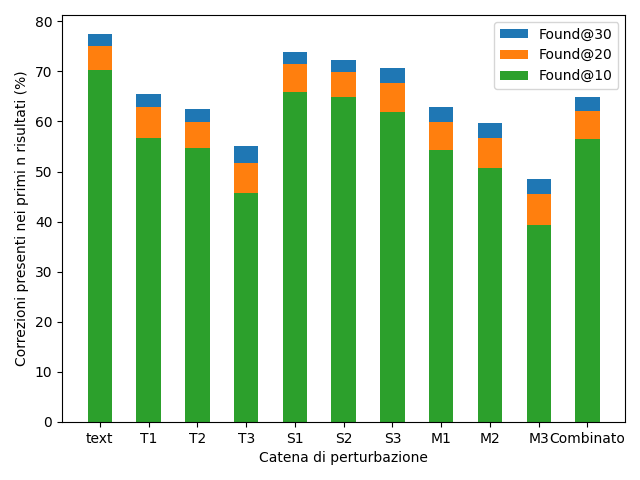
\includegraphics[width=.9\textwidth]{distributions/overview.png}
\caption{Correzioni presenti nei primi n risultati prodotti da BERT in percentuale}
\label{fig:foundN}
\end{figure}

Dai risultati è possibile trarre alcune conclusioni:
\begin{itemize}
\item BERT ottiene migliori performance nei testi ottenuti da pipeline con un più alto livello di perturbazione. Questo risultato è lecito da aspettarsi, in quanto le parole perturbate rendono meno intellegibile il contesto che BERT usa per produrre i candidati.
\item Mentre l'incremento delle correzioni corrette presenti nei candidati prodotti da BERT è sensibile  da 10 a 20 risultati, è praticamente trascurabile da 20 a 30 risultati.
\end{itemize}

Avendo stabilito la frequenza con la quale la giusta correzione è presente fra i candidati, è necessario che un sistema di correzione sia in grado di trovarla fra la varie alternative proposte.\\
A tale scopo è utile capire in quale posizione fra i risultati il token corretto si trovi. La distribuzione del posizionamento della soluzione è mostrata nel grafico in \autoref{fig:dis_pos}.

\begin{figure}[H]
\centering
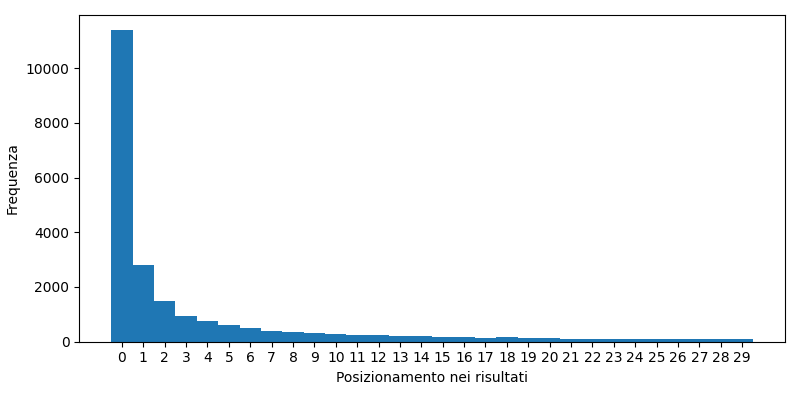
\includegraphics[width=\textwidth]{distributions/score_order_Combinato}
\caption{Distribuzione della soluzione nei primi 30 risultati}
\label{fig:dis_pos}
\end{figure}

Il grafico in \autoref{fig:dis_pos} è relativo al insieme combinato di tutte le frasi. Non vengono riportati i singoli grafici delle altre catene i perturbazione per brevità, in quanto sono praticamente sovrapponili a quello presente.\\
La distribuzione mostra come i risultati rilevanti si trovino a ridosso delle prime posizioni. Tuttavia, questa statista non basta per scegliere in modo affidabile il candidato per la correzione.


\section{Analisi prestazioni correttore}
In questa sezione sono misurate le prestazioni della parte di error correction relativa alla correzione dei singoli token del correttore sviluppato.

\subsection{Metodologia dell'analisi}
Per testare esclusivamente la parte di error correction viene usata una versione leggermente modificata del sistema di correzione sviluppato:
\begin{itemize}
\item La parte di error detection è completamente rimossa, in quanto non necessaria. Infatti, come visto in precedenza, in ogni frase l'errore da correggere è stato introdotto appositamente ed è già demarcato.
\item L'output del sistema non è l'intera frase con la correzione incorporata, ma solo la correzione proposta per il token errato.
\end{itemize}

Una correzione è considerata corretta solo se è esattamente identica alla parola originale.

\subsection{Metriche}
Per misurare quanto il sistema di correzione riesca ad approssimare il limite superiore di BERT sono introdotte le seguenti metriche:
\begin{itemize}
\item \textbf{Percentuale di scelta corretta:} per le correzioni nelle quali la soluzione è presente nei primi 20 risultati di BERT, è la percentuale di volte nelle quali il sistema è in grado di identificarla e sceglierla.
\item \textbf{Percentuale di falsi negativi:} per le correzioni nelle quali la soluzione è presente nei primi 20 risultati di BERT, è la percentuale di volte nelle quali il sistema trova la soluzione, ma la scarta perchè valutata troppo distante dalla parola da correggere.
\item \textbf{Percentuale di falsi positivi:} per le correzioni nelle quali la soluzione \textbf{non} è presente nei primi 20 risultati di BERT, è la percentuale di volte nelle quali il sistema sceglie comunque uno dei candidati, producendo un errore.
\end{itemize}


\subsection{Risultati}

Nella \autoref{tab:analisi_risultati} sono riportati i risultati per le metriche definite in precedenza.
\begin{table}[H]
\centering
\begin{tabular}{cccc}
\textbf{Perturbazione} & \textbf{Scelte Corrette} & \textbf{Falsi Negativi} &  \textbf{Falsi Positivi} \\ \hline
text& 88.16& 3.05& 27.28\\
T1& 86.41& 3.59& 32.29\\
T2& 83.97& 4.01& 32.2\\
T3& 80.17& 3.14& 35.16\\
S1& 86.93& 3.93& 27.25\\
S2& 87.85& 2.84& 28.04\\
S3& 86.41& 4.06& 29.86\\
M1& 85.03& 3.77& 31.63\\
M2& 84.07& 3.88& 32.53\\
M3& 80.29& 3.58& 40.35\\
Combinato& 85.3& 3.58& 32.5\\
\end{tabular}
\caption{Risultati sperimentali dell'error correction del sistema sviluppato}
\label{tab:analisi_risultati}
\end{table}

Come è lecito aspettarsi, i risultati sono tanto migliori quanto più basso è il livello di perturbazione.\\
Come visibile in \autoref{fig:torta_giuste}, oltre ai falsi negativi, il sistema sbaglia la soluzione nell'11\% delle correzioni. L'eventualità di una correzione sbagliata si presenta quando la soluzione non è la parola più vicina a quella da correggere nei risultati proposti da BERT. Ciò si può evincere anche dal grafico in \autoref{fig:lev_distribution}, dove si può notare come la grande maggioranza delle soluzioni sono il risultato più vicino alla parola da correggere.

\begin{figure}[H]
\centering
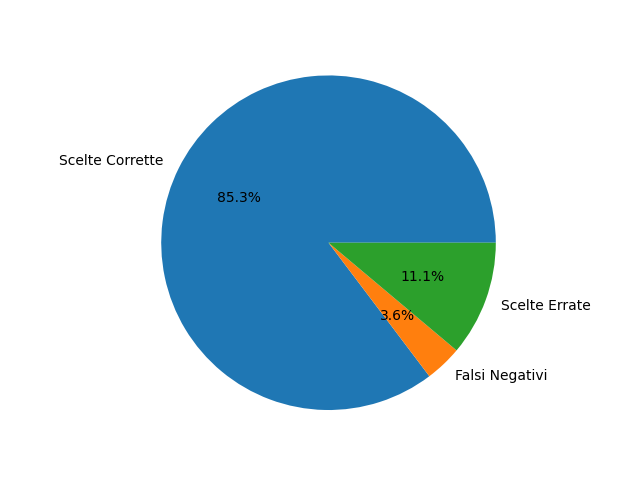
\includegraphics[width=\textwidth,trim={0 1.5cm 0 1.5cm},clip]{distributions/correct_combinato}
\caption{Scelte correte, scelte errate e falsi negativi relativi al combinato di tutti i livelli di perturbazione}
\label{fig:torta_giuste}
\end{figure}

\begin{figure}[H]
\centering
\includegraphics[width=\textwidth]{distributions/lev_pos_combinato}
\caption{Distribuzione dalla soluzione fra i risultati di BERT ordinati per la distanza di Levenshtein}
\label{fig:lev_distribution}
\end{figure}


In \autoref{fig:falsi_pos} invece si può vedere cosa succede in caso la soluzione non sia presente fra i primi 20 risultati: nel 67,5\% dei casi il sistema non effettua una correzione, mentre nel resto dei casi viene fornita una correzione errata.

\begin{figure}[H]
\centering
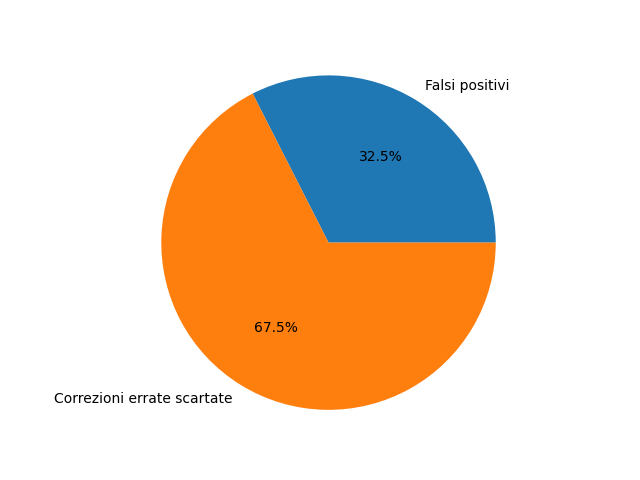
\includegraphics[width=\textwidth,trim={0 1.5cm 0 1.5cm},clip]{distributions/non_correct_combinato}
\caption{Falsi positivi e correzioni errate scartate relativi al combinato di tutti i livelli di perturbazione}
\label{fig:falsi_pos}
\end{figure}

Date queste statistiche, è possibile valutare in modo comprensivo il comportamento del correttore.\\
Vengono divise le scelte del correttore in due categorie:
\begin{itemize}
\item \textbf{Scelte positive}: distinguono i casi in cui il correttore sceglie la giusta soluzione se presente, o decide di non intervenire nel caso la soluzione non sia presente fra opzioni fornite da BERT.
\item \textbf{Scelte Negative}: distinguono i casi in cui il correttore sceglie una correzione sbagliata o decide di non intervenire in caso la soluzione sia presente fra i risultati di BERT. Sono inclusi anche i casi nei quali, in mancanza della soluzione fra i risultati, il correttore fornisce una correzione errata.
\end{itemize}

\begin{figure}[H]
\centering
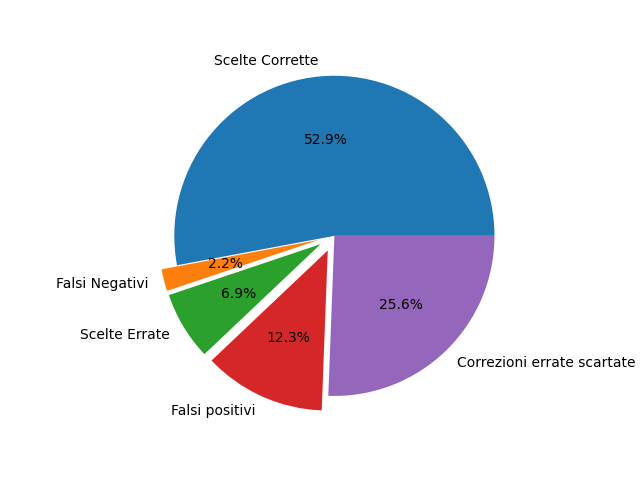
\includegraphics[width=\textwidth,trim={0 1.5cm 0 1cm},clip]{distributions/overview_scelte_combinato}
\caption{Scelte positive e negative relative al combinato di tutti i livelli di perturbazione. Nel diagramma, le scelte negative sono quelle distaccate dalla torta principale.}
\label{fig:scelte_pos_neg}
\end{figure}

Dal diagramma in \autoref{fig:scelte_pos_neg} si nota come il sistema di correzione faccia un scelta positiva nel 78\% dei casi.\\
In \autoref{tab:scelte_pos_neg} sono invece riportate le percentuali di scelte negative e positive per tutti i livelli di perturbazione.


\begin{table}[H]
\centering
\begin{tabular}{ccc}
\textbf{Perturbazione} & \textbf{\% Scelte Positive} & \textbf{\% Scelte Negative} \\ \hline
text& 84.29& 15.71\\
T1& 79.47& 20.53\\
T2& 77.5& 22.5\\
T3& 72.77& 27.23\\
S1& 82.88& 17.12\\
S2& 83.06& 16.94\\
S3& 81.14& 18.86\\
M1& 78.34& 21.66\\
M2& 76.87& 23.13\\
M3& 69.04& 30.96\\
Combinato& 78.55& 21.45\\
\end{tabular}
\caption{Percentuale di scelte positive e negative per tutti i livelli di perturbazione}
\label{tab:scelte_pos_neg}
\end{table}



%\begin{figure}[H]
%\centering
%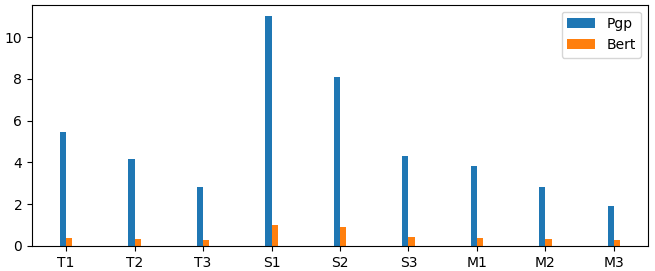
\includegraphics[width=\textwidth]{immagini/ipc}
%\caption{Rapporto fra gli errori erroneamente introdotti dal processo di correzione e gli errori corretti dallo stesso processo}
%\end{figure}


%\begin{table}[H]
%\centering
%\begin{tabular}{c|cc|cc|cc}
%& \multicolumn{2}{c}{\textbf{Metrica 1}} & \multicolumn{2}{c}{\textbf{Metrica 2}} & \multicolumn{2}{c}{\textbf{Metrica 3}} \\
%& Bert & Pgp & Bert & Pgp & Bert & Pgp \\ \hline
%T1 & 0.4 & 0.24 & 0.41 & 2.17 & 0.32 & 2.8 \\
%T2 & 0.4 & 0.27 & 0.42 & 2.15 & 0.26 & 1.96 \\
%T3 & 0.37 & 0.28 & 0.48 & 2.21 & 0.22 & 1.36 \\
%S1 & 0.27 & 0.15 & 0.36 & 2.0 & 0.91 & 9.38 \\
%S2 & 0.25 & 0.17 & 0.36 & 1.96 & 0.83 & 6.4 \\
%S3 & 0.28 & 0.16 & 0.39 & 1.8 & 0.44 & 3.53 \\
%M1 & 0.32 & 0.22 & 0.47 & 2.08 & 0.35 & 2.3 \\
%M2 & 0.33 & 0.25 & 0.47 & 2.0 & 0.26 & 1.49 \\
%M3 & 0.26 & 0.24 & 0.65 & 2.04 & 0.3 & 1.05 \\
%\end{tabular}
%\caption{Risultati sperimentali del correttore BERT e del correttore Pgp con frasi di lunghezza 100}
%\end{table}















\end{document}